%%%%%%%%%%%%%%%%%%%%%%%%%%%%%%%%%%%%
\chapter{Results}
\label{chap:Results}
%%%%%%%%%%%%%%%%%%%%%%%%%%%%%%%%%%%%
\comment{
The Results section should provide
\begin{itemize}
    \item An overview of all obtained results
    \item An in detail discussion/explanation of all results
    \item A scientific interpretation of the results
\end{itemize}


\section{Common attributes to pay attention to are:}
\begin{itemize}
    \item When comparing plots, keep the scale of axes consistent.  To do otherwise is misleading for the reader.
    \item If you are going to compare separate plots, consider if they can be better evaluated when combined into a single plot.
    \item When plotting data, particularly the \emph{mean}, ensure that you also plot error bars (or other method) of indicating the distribution.
    \item If a figure or plot is included, ensure it is referenced explicitly in the body text discussion.
    \item When a large table of data is included, consider whether it would be better communicated as a box-plot or something similar.
    \item All axes should be labelled and include units of measurement where applicable.
    \item All captions and figures should have captions with enough information to be understood at a glance.  Do not use captions to provide information that is better placed in the body text.  
    \item Remember to identify result outliers and anomalous data and to attempt an explanation or justification.
\end{itemize}

\
}


% 实验场景设置
\section{Experiment Design}

\subsection*{Map}
\label{chap:map}

% 本文中的所有实验在一张模拟库房场景的地图中进行。
All experiments in this paper were conducted on a map simulating a warehouse scenario.
% 此地图是从一组被广泛使用的benchmark中选出的。
This map was selected from a widely-used benchmark set\cite{stern2019mapf}\footnote{https://movingai.com/benchmarks/mapf.html} for testing, due to its appropriate size and obstacle distribution.

\begin{figure}[htbp]
    \centering
    \includegraphics*[width = \linewidth]{figures/map(color).png}
    \caption{The map used in the experiments. The outer border is not included in the map.}
    \label{fig:Map}
\end{figure}

% 地图的大小为161*63(外侧的框不是地图的一部分),图中的绿色代表障碍物,白色代表可通行。所有狭窄通道(边缘和障碍物之间的通道)均为一格/一像素宽。
The size of the map is 161$\times$63 (the outermost green frame is not part of the map), 
with green representing obstacles and white representing passable areas.
All narrow corridors (channels at the border and between obstacles) are one grid / pixel wide.

\subsection*{Agent Initialisation and Behaviour}
\label{chap:agent initialisation}
% agent的起点和终点是如何生成。。。
% 生成若干起点-终点对,保存为单独的文件,每次启动实验时从此文件中依次读入起点-终点对,并依次分配给启动的agent。
The starting points and their corresponding goal points for agents are pre-generated and stored in a launch file. 
During each experiment, all agents are started simultaneously, and then sequentially read the start-goal point pairs from this file and assign them to the agents as they are launched.
(e.g. if 50 agents are launched in a experiment run, the first 50 start-goal pairs are read from the launch file and assigned to the agents in order. The same approach is applied for different numbers of agents.)
% 如何生成的:
% 起点是位于地图最外圈的一圈可用位置(Fig4.1中的最外圈不是地图的一部分)。起点序列的顺序是随机打乱后存储在launch file中的。
The starting points are located in the outermost circle of the map (the outermost green obstacle border in Fig \ref{fig:Map} is not part of the map). The sequence of starting points is stored in the launch file after being randomly shuffled.
% 终点是跨过地图的另一侧,起点与终点的映射关系如下:
The goal points are on the opposite side of the map, and the mapping relationship between the starting points and the goal points is as follows:
\begin{align}
    x_{goal} = width(map) - x_{start}  \\
    y_{goal} = height(map) - y_{start} 
\end{align}

Where $x$ refers to the horizontal coordinate, and $y$ refers to the vertical coordinate.
% 这一映射的效果如下图所示:
The effect of this mapping is shown in the following figure:
\textbf{ADD PIC HERE} % 展示起点终点映射效果

% agent如何加入地图
% agent到达终点后的行为
% agent在成功加入网络后,尝试生成一个以给定起点起始的计划。若没有满足此要求的计划,则不存在于地图内(可视为在地图外等待)。
After successfully joining the network, the agent attempts to generate a plan starting from the given start. If no plan meeting this requirement is available, the agent is not present on the map (since the start is on the map boundary, it can be considered as waiting outside the map).
% 若在某时刻到达终点,则关机并从地图中消失(由于终点也位于地图边界,可视为退出地图)。
If the agent reaches the goal, it will shut down and disappear from the map (since the goal is also on the map boundary, it can be considered as exiting the map).

\subsection*{Parameters and Metrics}
% 算法共有四个参数:预测horizon,requied plan length, frame length, agent number
There are four adjustable parameters in the algorithm: 
\begin{enumerate}
    \item plan length limit: The upper limit of the length of the plan returned in a single planning session. Plans that exceed this length will be discarded.
    \item planning horizon: The upper limit of the future horizon that can be predicted in a single planning window, which is also the maximum length of the plan that can be generated in a single planning window.
    \item frame length: The length of the frame in the communication channel.
    \item agent number: The number of agents.
\end{enumerate}

There are five performance metrics:
\begin{enumerate}
    \item total path efficiency ratio: sum of actual path lengths / sum of optimal path lengths. 
    The optimal path is determined using A* algorithm under the assumption that there are no other agents present in the map.
    \item average path efficiency ratio: average of individual agents' (actual path length / optimal path length).
    \item final agent arrival time: the time at which the last agent reached its goal.
    \item average agent arrival time: the average arrival time for individual agents.
    \item average network join time: the average time spent by agents to join the network.
\end{enumerate}

\section{Experiment Results}
% 实验结果及讨论
% 数值结果
\subsection{Quantitative Results}

% 用数值化结果分析参数变化对系统性能的影响
Analyze the impact of parameter changes on system performance using quantitative results.


\subsubsection{plan length limit and planning horizon}

% 这两个参数主要影响生成的计划, plan length limit是返回计划长度的上限,planning horizon是可生成计划的上限
These two parameters mainly impact the generated plans. The plan length limit sets the global maximum length for the returning plans, while the planning horizon determines the upper length boundary for plans that can be generated.

% 其中,planning horizon是越长越好的,因为只有在这一范围内,agent才能做出有效行动,超出这一范围则只能执行默认行为(原地待机)。
A longer planning horizon is more favorable, as it allows agents to make effective actions within this range. Beyond this scope, agents can only execute default behaviour (remaining stationary) until next planning window arrive (see Section \ref{chap:model prediction}).

% plan length limit 在较长和较短时可能有不同的效果:
On the other hand, the plan length limit might have diverse effects when set to longer or shorter values:
\begin{itemize}
    \item When set to longer values: Sharing longer plans among agents, might enhance collaboration efficiency and overall effectiveness by enabling agents to coordinate over extended horizon.
    \item When set to shorter values: Sharing shorter plans among agents, could lead to more agile agent movements, potentially increasing efficiency by allowing for greater flexibility.
\end{itemize}

% 另外,plan length limit至少也应当等同于frame length, 因为计划长度短于一帧时agent会原地待机,极大降低效率。
Additionally, the plan length limit should be at least equal to the frame length. This is because when the plan length is shorter than one frame, the agent will remain stationary, significantly reducing efficiency.

% 为了验证上述猜想,进行两组实验如下:
To validate these hypotheses, two groups of experiments are conducted as follows:
\begin{itemize}
    % planning horizon = 30, plan length limit和frame length以10为步长遍历10-60的参数空间,其中plan length limit总是不小于frame length. agent number作为无关变量,保持和frame length相同。
    \item Group 1.1: agent number = frame length, planning horizon = 30, plan length limit and frame length explore a parameter space ranging from 10 to 60 in increments of 10. Notably, the plan length limit is always maintained to be greater than or equal to the frame length.
    \item Group 1.2: agent number = frame length, planning horizon = 60, plan length limit and frame length explore a parameter space ranging from 10 to 60 in increments of 10. Notably, the plan length limit is always maintained to be greater than or equal to the frame length.
\end{itemize}

% 实验中的随机因素是agent加入网络的时间,因为agent随机地选择信道中空闲槽位。
The random factor in the experiment is the time spent for agents to join the network, as agents randomly choose free slots in the channel when joining.
% 由于实验耗时较长(一槽对应1秒)对于参数空间中的每个点仅进行一次测试。
Due to the considerable time required for the experiment (one slot takes 1 second), each point in the parameter space is tested only once.
% 虽然这样无法排除部分随机性,但是实验结果中表明的趋势仍然是非常清楚的。
Although this approach doesn't eliminate all randomness, the trends indicated in the experimental results are still quite clear.

% 对于参数空间中的每个点仅


\begin{figure}[htbp]
    \centering
    \begin{subfigure}[t]{1.1\linewidth}
      \centering
      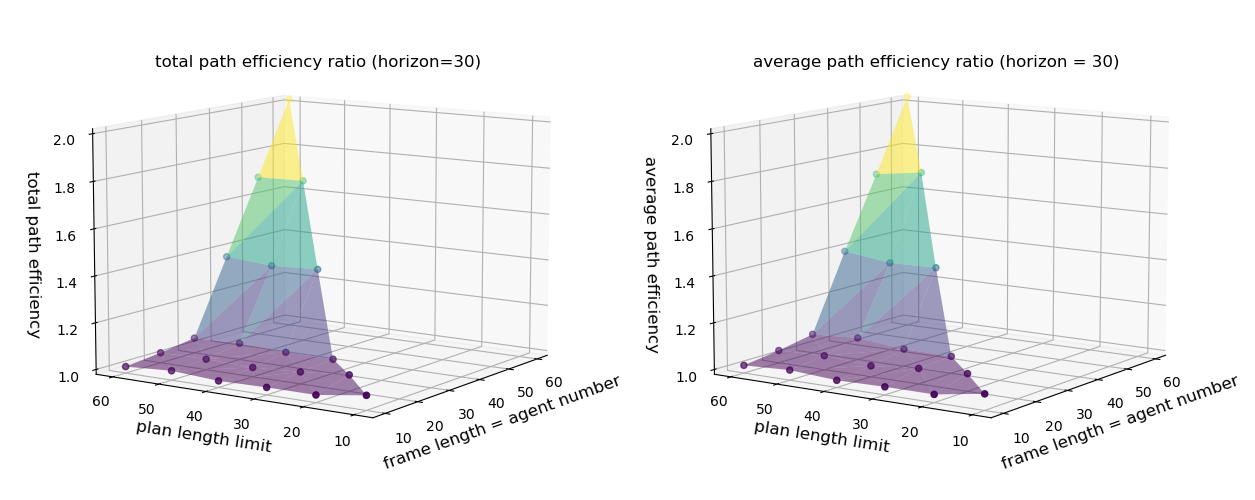
\includegraphics[width = \linewidth]{figures/horizon30_plan_length_limit_vs_performance.png}
      \caption{Experiment Group 1.1: path efficiency versus plan length limit (planning horizon = 30)}
      \label{fig:horizon=30,performance/planlengthlimit}
    \end{subfigure}
    \begin{subfigure}[t]{1.1\linewidth}
        \centering
        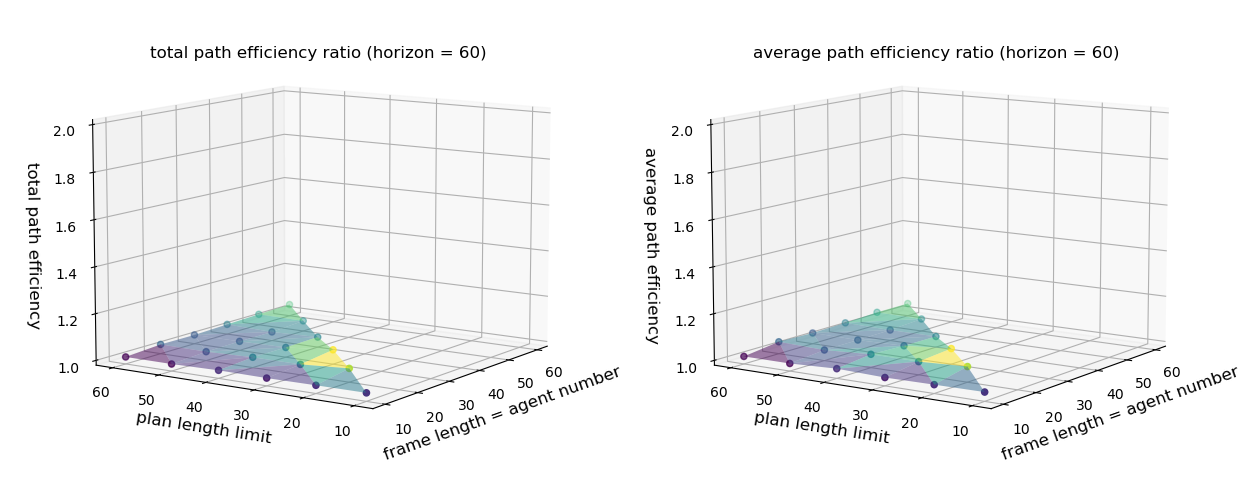
\includegraphics[width = \linewidth]{figures/horizon60_plan_length_limit_vs_performance.png}
        \caption{Experiment Group 1.2: path efficiency versus plan length limit (planning horizon = 60)}
        \label{fig:horizon=60,performance/planlengthlimit}
      \end{subfigure}
    \caption{Performance versus Planning Horizon and Plan Length Limit.}
    \label{fig:plan_length_limit}
\end{figure}

\FloatBarrier

% Fig4.2中展示了与路径质量相关的两个metric与planning horizon及plan length limit的关系。
In Figure \ref{fig:plan_length_limit}, the relationship between two metrics (total / average path efficiency) associated with path quality and the planning horizon, as well as the plan length limit, is illustrated.
% 结果可以分为两个部分:帧长度超出planning horizon的部分和帧长度未超出planning horizon的部分。
The results can be divided into two parts: the portion where the frame length exceeds the planning horizon, and the portion where the frame length does not exceed the planning horizon.

\begin{itemize}
    \item Frame length exceeds planning horizon: 
    
    % Fig 4.2.a中的斜坡部分就是这部分的结果。此部分中的frame lengt均大于planning horizon, 也就意味着在每帧的最后一部分,agent只能原地不动。
    The slope in Figure \ref{fig:horizon=30,performance/planlengthlimit} represents this segment of results. Within this portion, the frame lengths are all greater than the planning horizon, indicating that agents remain stationary during the final part of each frame.

    % 在这部分中,frame length和planning horizon的关系对路径效率起主导作用。可以看出,不论是总路径效率还是平均路径效率,都几乎等于帧长度与planning horizon的比例(如在frame length = 60处为2.0)
    In this section, the relationship between frame length and planning horizon predominantly influences path efficiency. It's evident that both the total path efficiency and the average path efficiency nearly equal the ratio of frame length to planning horizon (as seen at frame length = 60, the ratio is near 2.0, for instance).

    \item Frame length does not exceed planning horizon: 
    
    %Fig 4.2中所有剩余的平坦部分是这部分的结果。从图中可以看出,在frame length不超出planning horizon的情况下,路径效率几乎不随plan length limit变化。图中所有平坦部分的z轴(即metric)值均低于1.05.
    In Figure \ref{fig:plan_length_limit}, all the remaining flat sections represent the results of this segment. From the graph, it's evident that when the frame length does not exceed the planning horizon, path efficiency remains almost unchanged regardless of variations in the plan length limit. The z-axis values in all these flat sections of the graph are below 1.05.
    
    % 这表明:要么是plan length limit对路径效率没有显著影响,要么是地图对于实验中运行的agent来说过于开阔。
    This indicates that either the plan length limit has negligible impact on path efficiency, or the map is too open for the agents involved in the experiment. 

    % 对于地图太开阔的解释:如\ref{chap:map}中所提到的一样,虽然所有的走廊都只能有1agent宽,但由于障碍物的特殊分布,当一条路径被阻挡时,agent可以简单地选择在不同的路口转弯,来在不损失路径效率的情况下避开被使用的走廊。
    The explanation for the map being too open: 
    As mentioned in \ref{chap:map}, although all the corridors have a width of only one agent's width (one grid / pixel), due to the specific distribution of obstacles, 
    when a path is blocked, an agent can simply choose to turn at different intersections to avoid collision, 
    this allows them to avoid the occupied corridors without sacrificing path efficiency.
    % agent的起点终点设置\ref{chap:agent initialisation}可能加剧了这一情况,因为agent均需要跨过地图,而跨过此地图的最优路线有很多种。
    The setting of agent starting and ending points, as described in \ref{chap:agent initialisation}, might contribute to this situation. All agents need to cross the map, and there are many optimal routes for crossing this map, which could exacerbate the open nature of the map.
\end{itemize}

% 总体来说,实验结果表明,对于本测试情景,plan length limit并不重要。只要frame length不超出planning horizon, 路径效率就可以保持在接近最优的水平。
Overall, these experimental results indicate that, within the context of this test scenario, the plan length limit is not a critical factor. As long as the frame length does not exceed the planning horizon, path efficiency can be maintained at a level close to optimal.

\subsubsection{frame length and agent number}

% 这两组参数主要影响系统容量。frame length是一帧中槽的数量,agent number是同时启动agent的个数。
These two parameters are related to the system capacity. Frame length refers to the quantity of slots within a frame, while agent number represents the number of agents initiated simultaneously at the beginning of simmulation run.

% 帧长度较长和较短各有利弊。
The advantages and disadvantages exist for both longer and shorter frame lengths.
\begin{itemize}
    % 帧长度较长时,信道中有更多空间供agent使用,也就允许更多的agent加入信道。但若在加入过程中发生碰撞,根据协议,agent需要重听一整帧来重新确定分配情况来再次尝试加入,这一时长会随帧长度的增加而增加,因而帧长度并不是越长越好。
    \item Longer frame lengths:  there is more channel space available for agents, allowing a larger number of agents to join the channel. However, if collisions occur during the joining process, according to the protocol, agents need to re-listen to the entire frame to reconfirm the allocation and make another attempt to join. This time duration for re-listening increases with the longer frame length. Consequently, longer frame lengths do not necessarily lead to better outcomes.
    % 帧长度较短时,信道中空间不足,大量agent会停留在信道加入阶段,会导致效率的降低。此时虽然没有帧长度较长时重听一帧耗时长的弊端,但其信道容量本身就较低。
    \item Shorter frame lengths: When the frame length is shorter, there is limited channel space, which can result in a significant number of agents lingering in the channel joining phase. This can lead to reduced efficiency. Although this scenario may not suffer from the prolonged re-listening disadvantage seen with longer frame lengths, the inherent channel capacity is already low due to the shorter frame length.
\end{itemize}

% 从此处也可以看出,frame length的大小是相对于agent number的
From this perspective, it is apparent that the magnitude of the frame length is relative to the agent number.

% 为了验证帧长度的相对长短对系统性能的影响,进行如下实验:
To investigate the impact of varying frame lengths on system performance, the following experiments are conducted:

\begin{itemize}
    % 遍历以下的参数空间两次:planning horizon = 60, plan length limit = 60, agent number 10-60 步长为10,frame length 10-60 步长为5
    \item Group 2: The parameter space will be traversed twice with the following settings: planning horizon = 60, plan length limit = 60 (these two are independent parameters), agent number ranging from 10 to 60 with a step size of 10, and frame length ranging from 10 to 60 with a step size of 5.
    % 参数空间中的某些点由于耗时过长性能过差,予以省略
    Certain points in the parameter space (specifically, those with agent numbers significantly surpassing frame lengths) are omitted due to excessive time consumption and clearly inadequate performance.
\end{itemize}

% 实验中仍然存在与前一组实验相同的随机因素,即agent在加入信道时随机选择free slot尝试加入的这一因素。由于实验耗时比较可观(一个slot耗时1秒),仅遍历参数空间两次并取性能参数的平均值作为结果。虽然这样不能完全消除结果中的随机性,但性能随参数变化的趋势仍然表现得很明显。
Similar to the previous group of experiments, the same random factor exists in this group as well: the randomness associated with agents randomly selecting free slots to attempt joining the channel upon entry. 
Due to the considerable time required for the experiment (with each slot taking 1 second), the parameter space is traversed only twice, and the average values of performance metrics are taken as results. 
Although this approach doesn't entirely eliminate randomness from the outcomes, the performance trends with parameter variations are still quite evident.


\begin{figure}[htbp]
    \centering
    \begin{subfigure}[t]{0.45\linewidth}
      \centering
      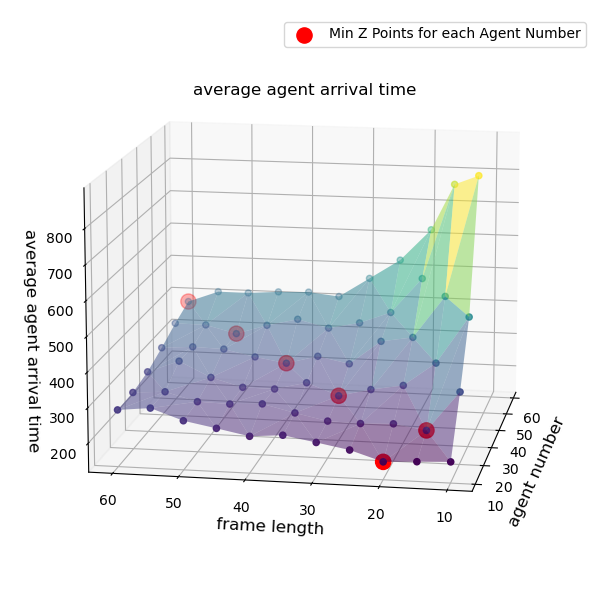
\includegraphics[width = \linewidth]{figures/avg_arrival_time.png}
      \caption{Average agent arrival time results}
      \label{fig:Performance1}
    \end{subfigure}
    \hfill
    \begin{subfigure}[t]{0.45\linewidth}
        \centering
        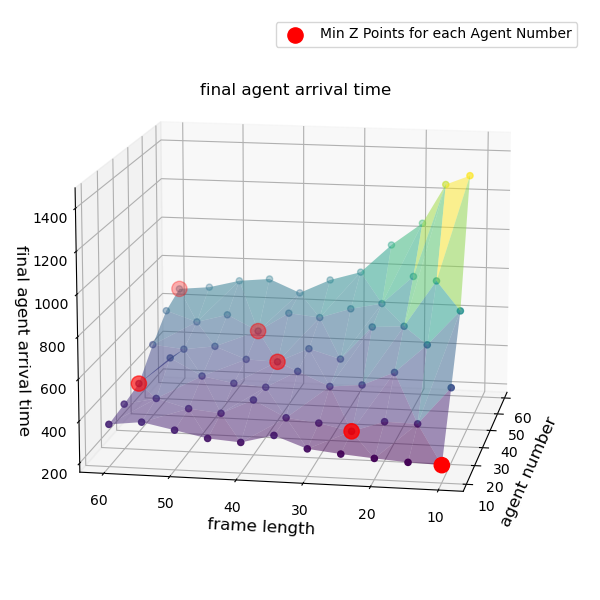
\includegraphics[width = \linewidth]{figures/final_agent_arrival_time.png}
        \caption{Final agent arrival time results}
        \label{fig:Performance2}
    \end{subfigure}
    
    \vspace{1cm}
    
    \begin{subfigure}[t]{0.45\linewidth}
        \centering
        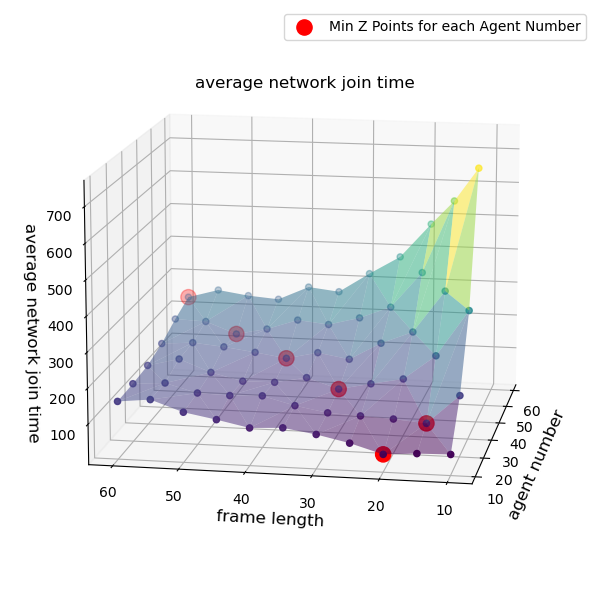
\includegraphics[width = \linewidth]{figures/avg_network_join_time.png}
        \caption{Average network join time results}
        \label{fig:Performance3}
    \end{subfigure}
    \hfill
    \begin{subfigure}[t]{0.45\linewidth}
        \centering
        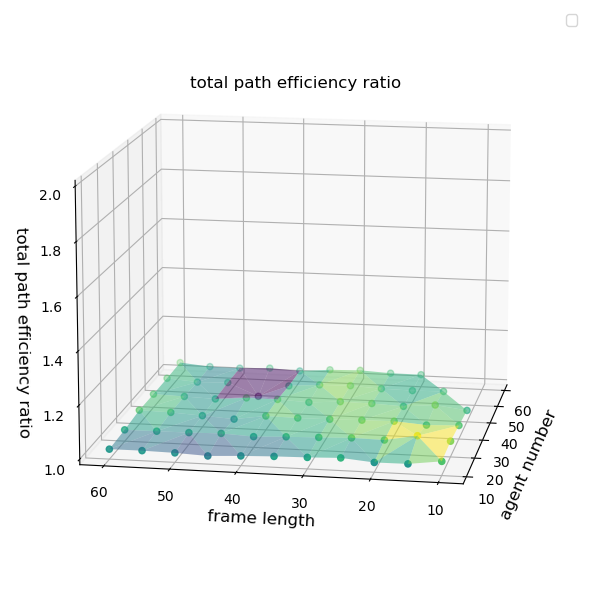
\includegraphics[width = \linewidth]{figures/total_path_effi_ratio.png}
        \caption{Total path efficiency ratio result}
        \label{fig:Performance4}
    \end{subfigure}
    \caption{Experiment Group 2: Performance versus agent number and frame length.}
    \label{fig:Performance}
\end{figure}
\FloatBarrier

% 能影响最重要的参数:arrival time的因素只有两个:(1)agent加入网络的耗时。(2)agent的路径效率。
There are only two factors that can influence the most important parameter, which is the arrival time. These factors are: (1) the duration it takes for an agent to join the network, and (2) the efficiency of the agent's path. 

% 而在这两个因素中,agent的路径效率在本实验场景中对arrival time的影响几乎没有,因为其本身在整个参数空间内的变化不大。
In these two factors, the path efficiency of the agent has almost no impact on the arrival time in this experimental scenario, as its variation across the entire parameter space is minimal.
% 从Figure \ref{fig:Performance4}可以看出,agent的路径效率始终保持在较高的水平(图中的所有点的z轴值均低于1.05,与第一组实验中的结果相同)
As can be seen from Figure \ref{fig:Performance4}, the efficiency of the agent's path is consistently high (all the points on the z-axis in the figure are below 1.05, which is in line with the results from the first group of experiments).
% Figure \ref{fig:Performance1,fig:Performance2,fig:Performance3}之间形状的相似也能证明这一点。虽然final arrival time由于更高的随机性(不像average arrival time那样由平均产生)而稍有走形,但其总体趋势仍然是一样的。
The similarity in shape between Figure \ref{fig:Performance1}, Figure \ref{fig:Performance2}, and Figure \ref{fig:Performance3} further supports this observation. While the final arrival time may deviate slightly due to higher randomness (as opposed to the average arrival time which is generated by averaging), the overall trend remains consistent.


% 因此,本实验场景中的性能参数主要由agent加入网络的耗时决定。性能在参数空间中的变化可以从这一方面来解释。
Consequently, the performance parameters in this scenario are primarily determined by the time it takes for an agent to join the network. The variation in performance across the parameter space can be explained from this perspective.


% 从图中可以看出,对于每个agent number,性能最优的点集中在agent number与frame length值接近或相等的地方。这一现象可以从以下两方面解释:
As can be seen from Figure \ref{fig:Performance1}, \ref{fig:Performance2}, \ref{fig:Performance3}, for each agent number, the points of optimal performance tend to concentrate where the agent number and frame length values are close or equal. 
% 以agent number = frame length的线为界,可以将结果分为两部分讨论:
Using the line where agent number = frame length as a reference, the results can be divided into two parts for discussion:

\begin{itemize}
    \item Agent Number < Frame Length:
    
    This part corresponds to the upper-right part of each figure in  Fig \ref{fig:Performance}. 
    When the agent number increases relative to the frame length, there is a significant negative impact on performance.
    
    % 这是因为此时信道容量过小,一部分agent必须待机,直到信道中有可用空间出现,才能开始运行。
    This is because, in this part, the channel capacity is relatively limited, and a portion of agents must remain idle until available channel space emerges, allowing them to start their operations.
    
    \item Agent Number > Frame Length
    
    This part corresponds to the bottom-left part of each figure in Fig \ref{fig:Performance}. 
    As the frame length increases relative to the agent number, the performance gradually declines.
   

    % 此时,channel的容量允许全部agent在网络中运行,但是根据协议,若多个agent在尝试加入网络时发生碰撞(碰巧尝试占用同一个空闲槽位),则在下一次尝试之前必须听完完整的一帧。这一机制使得过长的frame length对agent join time有负面影响。
    In this part, the channel has enough capacity for all the agents to operate in the network at same time. 
    However, according to the protocol, if multiple agents collides in the channel (accidentally trying to occupy the same free slot when entering), they must wait and listen through an entire frame before attempting again. This mechanism means that an excessively long frame length has a negative impact on the agent join time.

\end{itemize}


% 这就可以理解为什么对于每个agent number来说,性能最优的点大多是frame length = agent number或稍高于 agent number。因为此时信道中有足够的位置,不会出现只能待机的agent,同时帧长度又没有过长,加入网络中重试的过程不会耗时过长。
This explains why, for each agent number, the points with the optimal performance are mostly when the frame length equals the agent number or slightly higher than the agent number. In these cases, there is enough room in the channel to avoid having agents solely in idle mode, while the frame length is also not excessively long, preventing a prolonged process of retrying to join the network.

\comment{
\textbf{Proportion of Agents in Channel versus Time}

% 基于stdma的agent对channel的利用率也影响了系统的性能,因为在本文的算法中,只有在channel中的agent才能在地图中移动(见 Section \ref{chap:join map})。
The proportion of agents in the channel also affects the system's performance. In the algorithm proposed in this study, only the agents present in the channel are able to move within the map, as discussed in Section \ref{chap:join map}.
% 这与上述"只有两个因素影响性能"的结论不矛盾,因为信道使用率可以看作agent join time的另一种表现方式。
This is consistent with the conclusion mentioned above that only two factors impact performance, as this can be viewed as another manifestation of network join time.

% 为了分析agent number和frame length对信道的利用情况的影响,从Exeriment Group2中进行的两次重复实验中选出一次,将每个agent number对应不同frame length时,信道中agent的数量与时间的关系绘制出来。为了使结果在图中清晰一些,frame length不为10的倍数的部分数据没有被画出。
To analyze the proportion of agents in channel, select one of the two repetitions conducted in Experiment Group 2. 
For each agent number at different frame lengths, create a graph that illustrates the relationship between the percent of agents in the channel and time. 
To enhance clarity in the graph, data points where frame length is not a multiple of 10 are excluded from the representation.

% 注意,agent在到达终点后会关机并放弃自己在信道中的槽。
Notably, agents shut down and release their slots in the channel upon reaching their goals (see Section \ref{chap:exit map}).
% 所有agent都退出信道时,就说明所有agent都已经到达终点。
When all agents have exited the channel, it indicates that all agents have reached their goals.


\begin{figure}[htb]
    \centering
    % Row 1
    \begin{subfigure}[t]{0.45\linewidth}
        \centering
        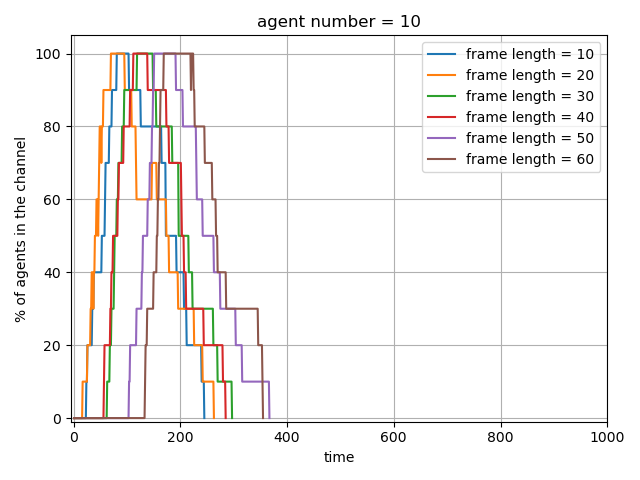
\includegraphics[width=\linewidth]{figures/channel_usage_agent10.png}
        \caption{10 agents}
        \label{fig:agentpercent1}
    \end{subfigure}
    \hfill
    \begin{subfigure}[t]{0.45\linewidth}
        \centering
        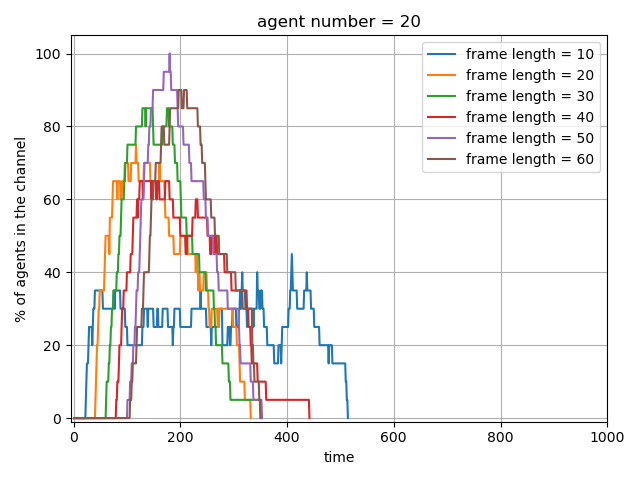
\includegraphics[width=\linewidth]{figures/channel_usage_agent20.png}
        \caption{20 agents}
        \label{fig:agentpercent2}
    \end{subfigure}
    
    \vspace{1cm}
    
    % Row 2
    \begin{subfigure}[t]{0.45\linewidth}
        \centering
        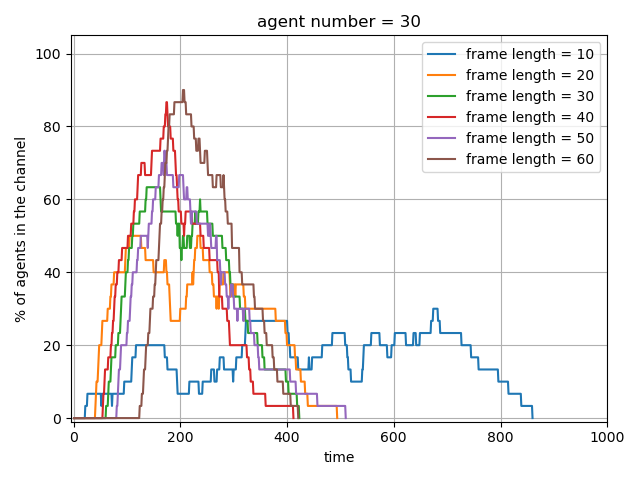
\includegraphics[width=\linewidth]{figures/channel_usage_agent30.png}
        \caption{30 agents}
        \label{fig:agentpercent3}
    \end{subfigure}
    \hfill
    \begin{subfigure}[t]{0.45\linewidth}
        \centering
        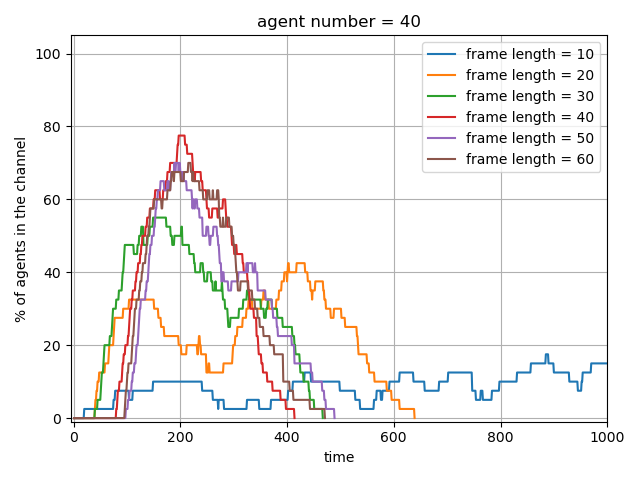
\includegraphics[width=\linewidth]{figures/channel_usage_agent40.png}
        \caption{40 agents}
        \label{fig:agentpercent4}
    \end{subfigure}
    
    \vspace{1cm}
    
    % Row 3
    \begin{subfigure}[t]{0.45\linewidth}
        \centering
        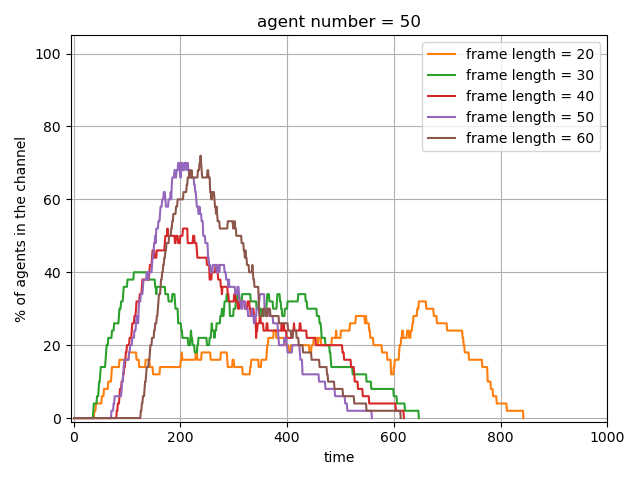
\includegraphics[width=\linewidth]{figures/channel_usage_agent50.png}
        \caption{50 agents}
        \label{fig:agentpercent5}
    \end{subfigure}
    \hfill
    \begin{subfigure}[t]{0.45\linewidth}
        \centering
        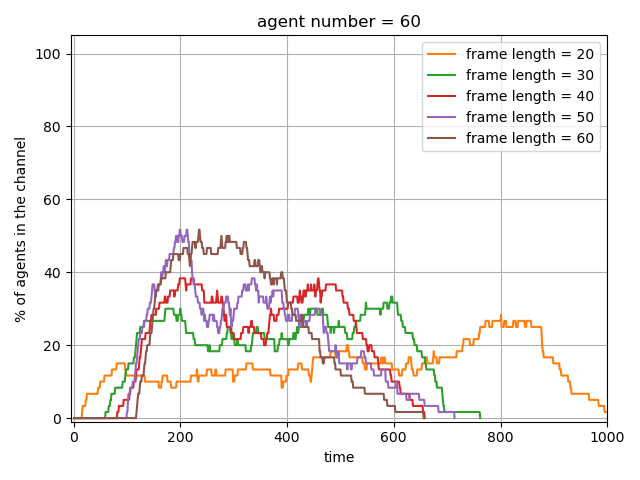
\includegraphics[width=\linewidth]{figures/channel_usage_agent60.png}
        \caption{60 agents}
        \label{fig:agentpercent6}
    \end{subfigure}
    
    \caption{Graph illustrating the relationship between the percentage of agents in the channel and time for different agent numbers at various frame lengths.}
    \label{fig:grid}
\end{figure}




% 对实验结果的一些观察:
\begin{itemize}
    % agent number << frame length时,帧长度越短,全部agent进入网络越快。证据: 图一的峰值顺序
    \item 1
    % agent number < frame length时,frame length越短,channel utilization越高。证据:
    \item 2
    \item 3
    \item 4
    \item 5
\end{itemize}

}

% 在某些场景中的行为
\subsection{Deadlock Situation}

A deadlock situation arises only under exceptionally strict conditions.

\subsubsection{Condition}
% 满足下述情况时,agent之间发生死锁:
When the following conditions are simultaneously met, a deadlock between agents occurs:

\begin{enumerate}
    \item Two agents are positioned within a sufficiently long corridor that's only one agent wide, each agent starts from different sides of the corridor and needs to reach the opposite end of this corridor.
    % agent发布计划的长度必须大于等于frame length
    \item The length of plans published by agents = frame length, i.e., planning horizon $\geq$ frame length and plan length limit = frame length.
    % 当一方开始计划时,另一方的计划应当执行了半frame length长度,而剩余半frame length的计划中包含正在计划的一方的当前位置或当前位置的相邻点,且另一方的计划为向自己的目的地前进。
    \item When one agent begins its planning, the other agent's plan should already be halfway executed, 
    with only half a frame length remaining. 
    \begin{itemize}
        \item This yet-to-be-executed half of the plan should contain the current or adjacent position of the planning agent, which means this yet-to-be-executed part interferes the new plan of the planning agent. 
        \item The content of this half frame length plan should be solely directed towards its goal (advancing).
    \end{itemize}
\end{enumerate}
% 解释:为什么此种情况会发生死锁
\subsubsection{Explanation}

% 由于stdma的特性,两个agent的计划是轮流制订的,因为它们的计划时间窗就是它们的slot。同时,agent每次发布的计划长度是全局一致的。
Because the characteristic of STDMA, the two agents make plan in turns, as their planning time window is their slot in the repeating frame.
Additionally, agents publish plans of the same length throughout the entire system (see Section \ref{chap:model prediction}).

% 在这一情况下,agent的计划可以分为两部分:
In this scenario, an agent's plan could be divided into two parts:
\begin{itemize}
    % 1. 后退:受到无碰撞约束的影响,当对方在计划中前进时必须后退
    \item Retreating: Due to collision-free constraints, when the other agent is moving forward in its plan, the agent must retreat to avoid collision.
    % 2. 前进:己方计划时,在planning horizon的后面,对方的计划已用尽,这时可以不受对方计划的影响而前进。
    \item Advancing: When planning and in the later part of the planning horizon, the other agent's plan has exhausted (and at this point, the planning agent doesn't assume that another agent will idle after its plan ends, because a sufficient plan has already been published for it to use until its next planning window.). The planning agent could fill the rest part of its new plan with actions of proceeding toward its goal.
\end{itemize}

% 当前进和后退两部分长度相等时,就会陷入一种动态的死锁:双方各自花一半的计划用于前进,另一半用于后退。
When the lengths of the advancing and retreating segments are equal, a dynamic deadlock scenario emerges: 
both agent spend half of their plans for advancing and the other half for retreating.



\begin{figure}[htbp]
    \centering
    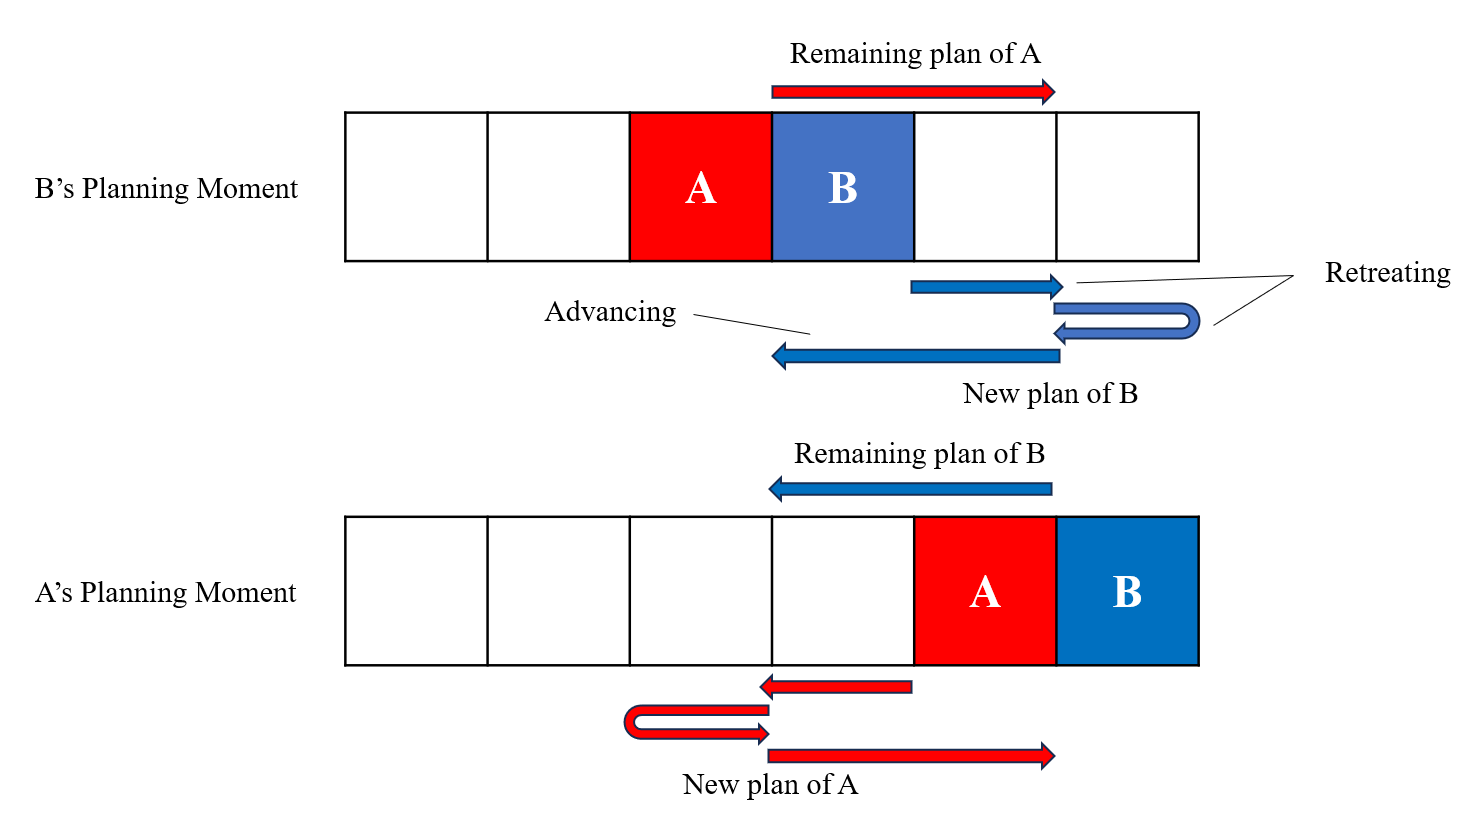
\includegraphics[width = \linewidth]{figures/deaclock_1.png}
    \caption{Example of a deadlock situation (frame length = 4, agent publishes plan with a length of 4).}% 死锁情况示例。(frame length = 4)
    \label{fig:deadlock}
\end{figure}
\FloatBarrier

\subsubsection{Solution}

% 由于此死锁情景的苛刻要求,只要打破条件1,2,3中的任意一个即可。
Due to the stringent requirements of this deadlock scenario, breaking any one of the three conditions will suffice.

For example:
\begin{itemize}
    \item Use odd-numbered frame length: This breaks the tie between advancing and retreating, because these two parts cannot be of equal length.
    \item Avoid using long narrow corridors: Add additional area to the corridor, don't force agents to push each other.
    \item Allow agents to publish longer plans:
     % 因为一方提前预定了很长空间用于前进,另一方必须在计划中对应的部分后退,这使得前进-后退的循环非常不均衡,从而可以快速离开走廊区域。
     If one agent requests an extensive span of space in their plan for advancing, the other agent will be compelled to retreat in the corresponding part of its plan. This results in a highly imbalanced advance-retreat cycle, facilitating a swift exit from the corridor area.
\end{itemize}

% 此情景在生成量化结果时未出现,因为测试地图中的障碍物相对于测试中使用的planning horizon足够小,且此情景本身出现条件比较苛刻。
This situation didn't show up in the quantitative result generating. This is mostly because the obstacles on our test map were relatively small compared to the planning horizon applied, so one agent could book all space in the corridor for advancing in one plan. Also, the conditions for this situation is quite strict.

\subsection{Failure Situation}

In the deadlock scenario, if there is a third agent, it could result in a failure: agent in the middle cannot find any possible plan.

\subsubsection{Condition}

\begin{enumerate}
    \item Three agents are positioned within a sufficiently long corridor that's only one agent wide.
    \item All agents are trying to get from one side of the corridor to the other, and one agent's starting and ending points are the complete opposite of the other two agents' starting and ending points.
\end{enumerate}

\begin{figure}[htbp]
    \centering
    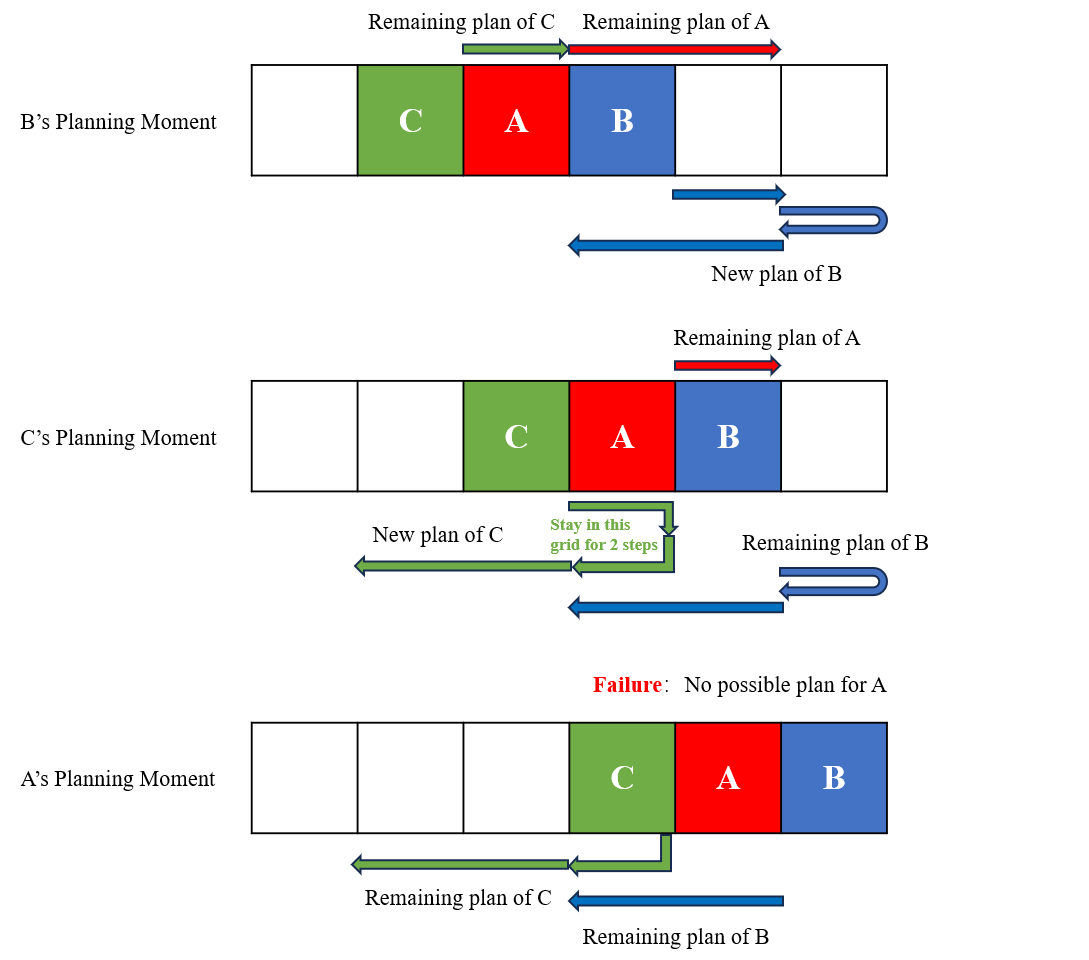
\includegraphics[width = \linewidth]{figures/Failure.png}
    \label{fig:failure}
    \caption{Example of failure. Due to the squeeze of agent C, agent A cannot find any possible plan (frame length = 4, agent publishes plan with a length of 4).}
\end{figure}

\subsubsection{Explanation}

% 此情况发生的主要原因是位于同一侧的两个agent之间的冲突。
The primary reason this situation arises is due to the conflict between the two agents on the same side of the corridor.
% 由于agent顺序计划,总会发生如下情景:
Since agents plan sequentially, the following scenario will always occur among the two agents on the same side:
\begin{itemize}
    \item 
    % 位于最外侧的agent在计划时,内侧的agent计划用尽,于是外侧agent认为可以继续前进,从而前进到与对侧agent相邻的位置
    When the outermost agent (C in Fig \ref{fig:deadlock}) is planning, the inner agent's plan exhaust within the planning horizon, leading the outermost agent to believe it can keep moving forward, subsequently advancing to a position adjacent to the agent on the opposite side.
    \item 
    % 当内侧的agent(也就是三个agent中位于中间的agent)进行计划时,由于外侧agent的挤压,无足够空间供其使用。
    When the inner agent (A in Fig \ref{fig:deadlock}, the one in the middle of the three agents) plans next, there isn't enough space for it due to the squeeze from the outer agent.
\end{itemize}

\subsubsection{Solution}

\begin{itemize}
    \item
    When the plan length that an agent can publish is sufficiently long relative to the length of the corridor, allowing an agent to reserve most of the space in the corridor in advance for its progression can prevent this situation (as seen in previous experiments where this situation didn't arise).
    \item 
    Modify the consensus among agents. Currently, an agent only assumes other agents will remain stationary after their plans run out if the published plan length of the other agents is less than one frame (see Section \ref{chap:model prediction}). If, during planning, agents always assume that other agents will stay in place once their plans are exhausted, this situation can be avoided. However, it might lead to potential decreases in path efficiency.
    \item 
    Avoid using overly long narrow corridors.
\end{itemize}


\subsection{Local Optimal Trap}

% 当障碍物足够大,agent在单个planning horizon 无法越过时,则会陷入一个局部最优陷阱中。
When an obstacle is sufficiently large such that an agent cannot surpass it within the planning horizon, the agent can become ensnared in a local optimal trap.
% agent会在障碍物内侧离终点最近的位置上保持静止,因为无法在单个planning horizon中到达比此点更接近终点的点。
The agent will remain stationary at the position inside the obstacle that is closest to the goal, as it cannot reach a position closer to the goal within a single planning horizon.

% 这是因为每次agent计划时都仅遍历一定horizon内的可能计划,然后选择这些计划中最后位置离终点最近的。
This occurs because each time the agent plans, it only explores potential plans within a certain horizon and then selects the one where the final position is closest to the goal.
% 如果horizon足够长,则可以克服此问题
If the planning horizon is long enough, this problem could be overcome.

\begin{figure}[htbp]
    \centering
    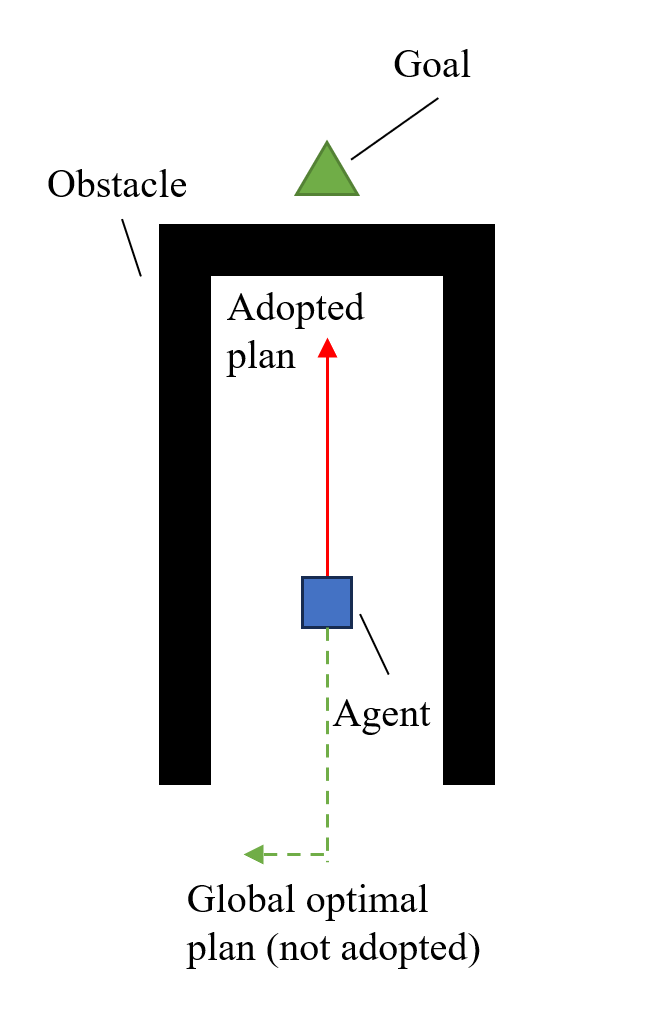
\includegraphics[width = 0.34\linewidth]{figures/Local Optimal Trap.png}
    \label{fig:LocalOptimalTrap}
    \caption{An agent trapped in a local optimum due to a short planning horizon, preventing its arrival.}% agent由于planning horizon较短,陷入局部极值陷阱并无法离开
\end{figure}
\FloatBarrier

This situation didn't show up in the quantitative result generating. This is mostly because the obstacles on our test map were relatively small compared to the planning horizon applied.

\subsection{Channel Utilization}

% 对于使用stdma分享信道的agent来说,信道并不总是满的。实际上,信道的一部分总是被许多未能获得槽的agent争抢,它们在其中相互碰撞。
For agents using STDMA to share channels, the channels aren't always full. In fact, a portion of the channel is always contended for by numerous agents that haven't secured a slot, leading to mutual collisions among them.
% 我们通过观察不同agent数量下信道的使用率来分析此问题。
We analyze this issue by observing the channel usage rate with varying numbers of agents.

\begin{figure}[htbp]
    \centering
    % Row 1
    \begin{subfigure}[t]{0.45\linewidth}
        \centering
        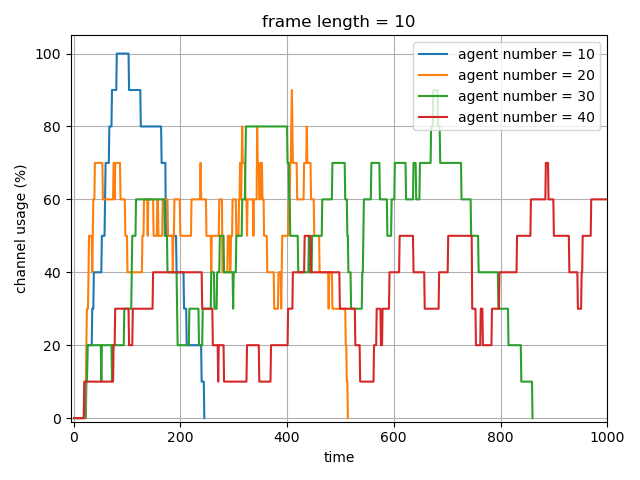
\includegraphics[width=\linewidth]{figures/channel_usage_frame10.png}
        \caption{frame length = 10}
        \label{fig:framepercent1}
    \end{subfigure}
    \hfill
    \begin{subfigure}[t]{0.45\linewidth}
        \centering
        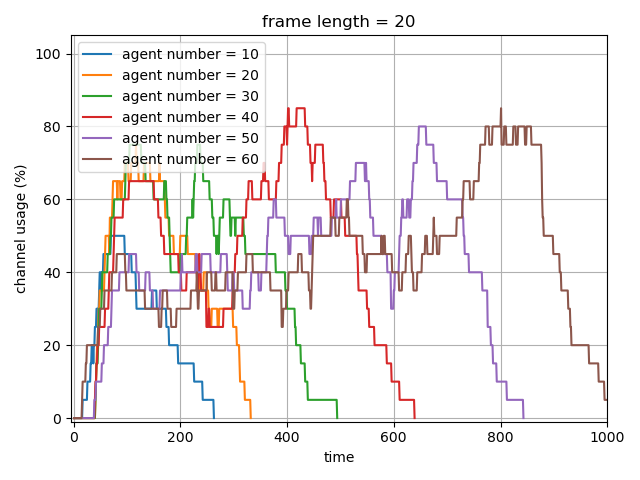
\includegraphics[width=\linewidth]{figures/channel_usage_frame20.png}
        \caption{frame length = 20}
        \label{fig:framepercent2}
    \end{subfigure}
    
    \vspace{1cm}
    
    % Row 2
    \begin{subfigure}[t]{0.45\linewidth}
        \centering
        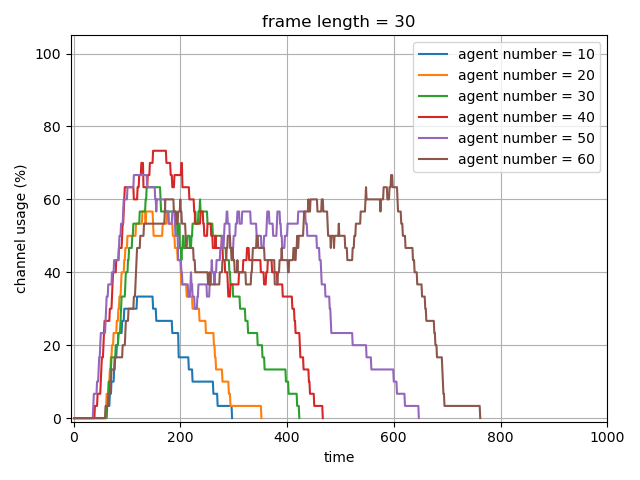
\includegraphics[width=\linewidth]{figures/channel_usage_frame30.png}
        \caption{frame length = 30}
        \label{fig:framepercent3}
    \end{subfigure}
    \hfill
    \begin{subfigure}[t]{0.45\linewidth}
        \centering
        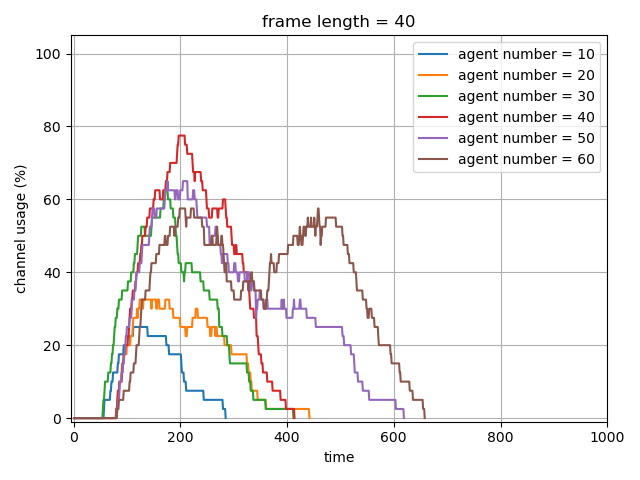
\includegraphics[width=\linewidth]{figures/channel_usage_frame40.png}
        \caption{frame length = 40}
        \label{fig:framepercent4}
    \end{subfigure}
    
    \vspace{1cm}
    
    % Row 3
    \begin{subfigure}[t]{0.45\linewidth}
        \centering
        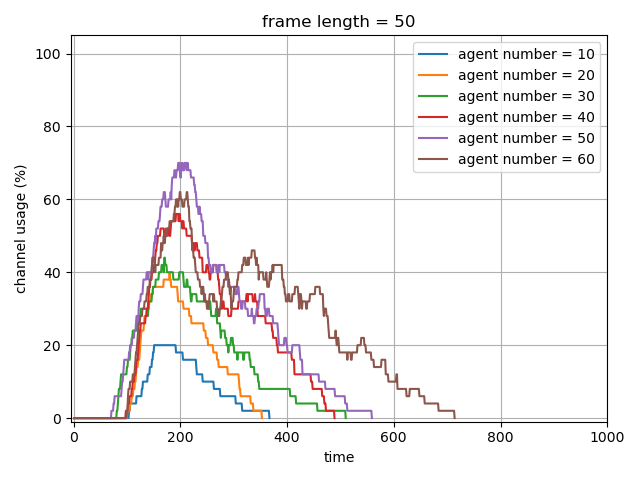
\includegraphics[width=\linewidth]{figures/channel_usage_frame50.png}
        \caption{frame length = 50}
        \label{fig:framepercent5}
    \end{subfigure}
    \hfill
    \begin{subfigure}[t]{0.45\linewidth}
        \centering
        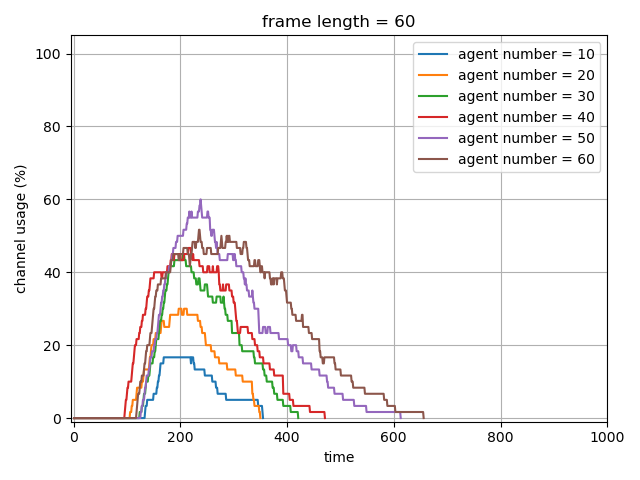
\includegraphics[width=\linewidth]{figures/channel_usage_frame60.png}
        \caption{frame length = 60}
        \label{fig:framepercent6}
    \end{subfigure}
    
    \caption{Graph illustrating the relationship between the percentage of channel usage and time for different agent numbers.}
    \label{fig:channelpercent}
\end{figure}


% 2. 信道使用率最高在80%左右(除去Figure \ref{fig:framepercent1}中10 agent, frame length = 10这种小规模的情况)。
% 3. agent数量越是与frame length接近,对信道的使用率越高。可以从两方面看出这一点:
%    - 最先达到峰值的是与frame length较接近的agent number的曲线
%    - 若agent number大大超过frame length,则此组对于信道的使用率会逐渐上升,因为完成任务的agent逐渐下降,系统中的活动agent数量减少,使其逐渐接近agent number = frame length。
% 从Figure \ref{fig:channelpercent}中,可以看出以下几条:
From Figure \ref{fig:channelpercent}, we can deduce the following points:
\begin{enumerate}
    \item 
    The highest channel usage rate is around 80\%, excluding small-scale scenarios like 10 agents with a frame length of 10 as seen in Figure \ref{fig:framepercent1}.
    \item 
    The channel usage rate is higher when the number of agents is closer to the frame length. This can be observed in two ways:
    \begin{itemize}
        \item 
        The first curves in each figure to reach their peak are those where the number of agents is closer to the frame length.
        \item
        If the number of agents far exceeds the frame length (e.g., Fig \ref{fig:framepercent2}, \ref{fig:framepercent3}), the channel usage rate for this group gradually increases. This is because the number of agents completed tasks rises, reducing the number of active agents in the system, making it gradually approach the scenario where the number of agents equals the frame length.
    \end{itemize}
\end{enumerate}


\subsection{Portion of Agents in Channel}

% 在本算法的条件下,只有在信道中的agent才可以发布计划并在地图中运动,因此在信道中的agent的比例值得关注。
% 我们通过观察不同frame length下agent在信道中的比例来观察此问题。
In the implemented algorithm, only agents present in the channel can publish plans and move within the map. Hence, the proportion of agents in the channel is worthwhile to take a look.
We delve into this matter by analyzing the proportion of agents in the channel across different frame lengths.

\begin{figure}[htbp]
    \centering
    % Row 1
    \begin{subfigure}[t]{0.45\linewidth}
        \centering
        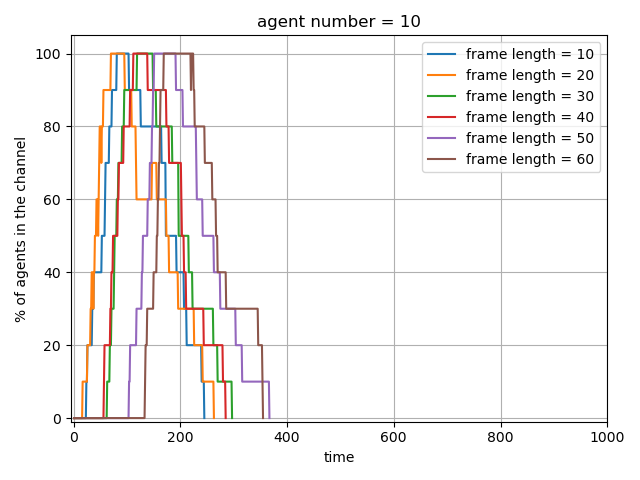
\includegraphics[width=\linewidth]{figures/channel_usage_agent10.png}
        \caption{10 agents}
        \label{fig:agentpercent1}
    \end{subfigure}
    \hfill
    \begin{subfigure}[t]{0.45\linewidth}
        \centering
        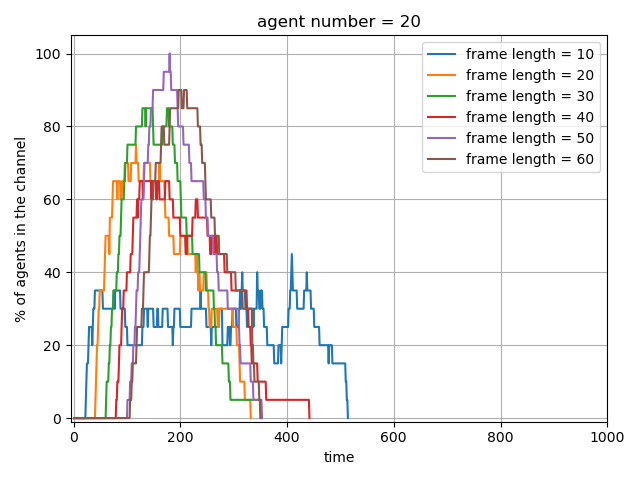
\includegraphics[width=\linewidth]{figures/channel_usage_agent20.png}
        \caption{20 agents}
        \label{fig:agentpercent2}
    \end{subfigure}
    
    \vspace{1cm}
    
    % Row 2
    \begin{subfigure}[t]{0.45\linewidth}
        \centering
        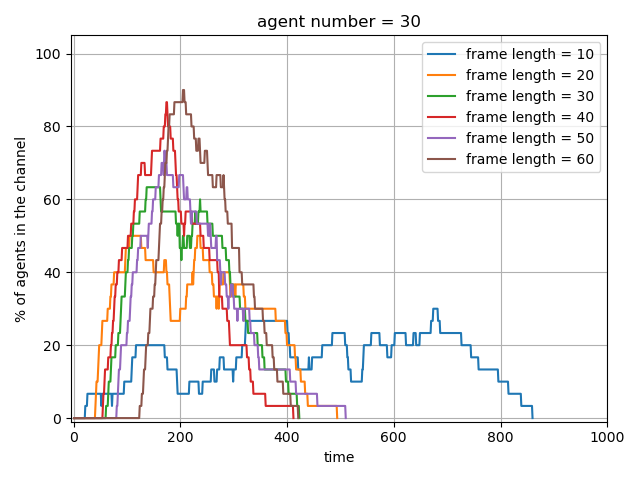
\includegraphics[width=\linewidth]{figures/channel_usage_agent30.png}
        \caption{30 agents}
        \label{fig:agentpercent3}
    \end{subfigure}
    \hfill
    \begin{subfigure}[t]{0.45\linewidth}
        \centering
        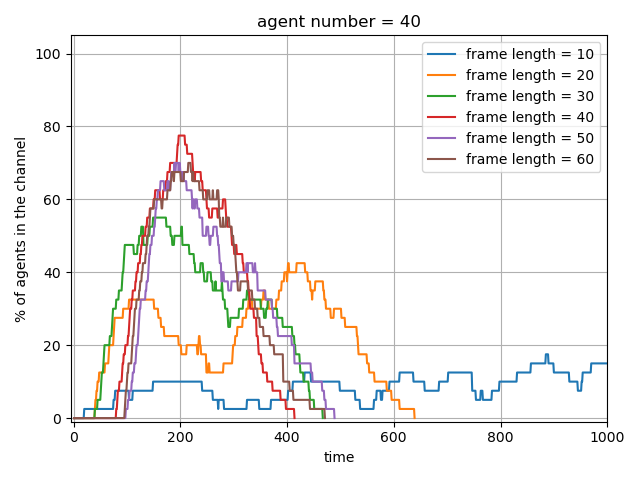
\includegraphics[width=\linewidth]{figures/channel_usage_agent40.png}
        \caption{40 agents}
        \label{fig:agentpercent4}
    \end{subfigure}
    
    \vspace{1cm}
    
    % Row 3
    \begin{subfigure}[t]{0.45\linewidth}
        \centering
        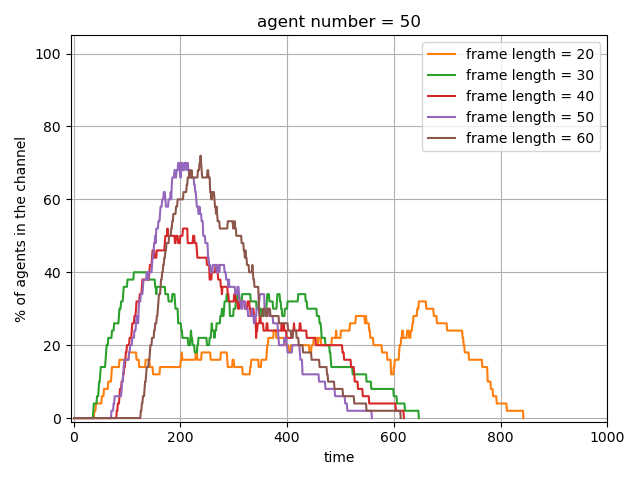
\includegraphics[width=\linewidth]{figures/channel_usage_agent50.png}
        \caption{50 agents}
        \label{fig:agentpercent5}
    \end{subfigure}
    \hfill
    \begin{subfigure}[t]{0.45\linewidth}
        \centering
        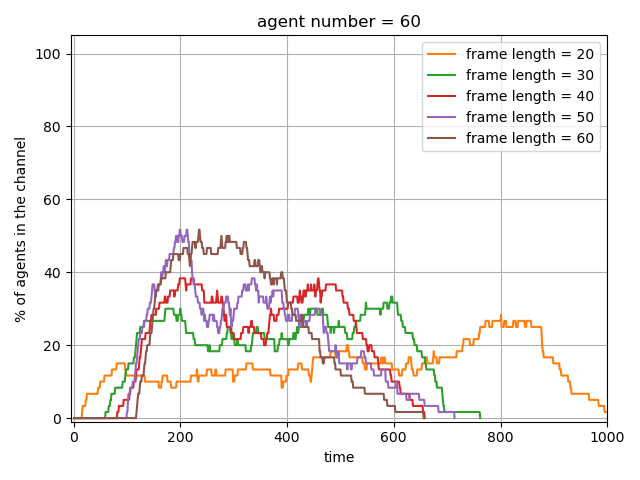
\includegraphics[width=\linewidth]{figures/channel_usage_agent60.png}
        \caption{60 agents}
        \label{fig:agentpercent6}
    \end{subfigure}
    
    \caption{Graph illustrating the relationship between the percentage of agents in the channel and time for different agent numbers at various frame lengths.}
    \label{fig:agentpercent}
\end{figure}

% 从Figure \ref{fig:agentpercent}中,可以得到以下信息:
From Figure \ref{fig:agentpercent}, we can deduce the following points:
\begin{enumerate}
    \item 
    % 1. 当frame length高于agent number时,可以允许更多的agent同时存在于信道中,但帧越长,agent加入信道的耗时就越长,在图中表现为达到峰值较慢,如 Fig \ref{fig:ageentpercent1}中,虽然所有frame length都可以使全部agent进入channel, 但是frame length越长,达到峰值越慢。
    When the frame length significantly exceeds the agent number, more agents can enter the channel. However, the longer the frame, the more time it takes to reach the peak percentage, manifesting as a slower rise to peak values in the graph (e.g., Fig \ref{fig:agentpercent1}).
    \item 
    % 2. 当agent number 超过frame length时,在信道中的agent数量显著减少,不只是因为帧中没有足够的空间,也因为有太多的agent争抢空闲槽位。随着agent逐渐减少(陆续完成任务),信道中的agent数量反而提升(e.g., Fig \ref{fig:agentpercent3} 中frame length = 20的曲线)
    When the agent number surpasses the frame length, the portion of agents in the channel drops notably. This decrease isn't solely due to the lack of enough space in the frame but also because too many agents are contending for the available slots. As agents progressively decrease (as they complete their tasks over time), the number of agents in the channel increases (e.g., the curve for frame length = 20 in Fig \ref{fig:agentpercent3}, \ref{fig:agentpercent4}, \ref{fig:agentpercent5}, \ref{fig:agentpercent6}).
    \item 
    % 3. 当frame length在agent number左右的时候,在信道中的agent的百分比的峰值大约保持在60%左右,这一值随着frame length增加而上升,随frame length减少而减少。
    When the frame length is around the same as the agent number, the peak percentage of agents in the channel stabilizes at around 60\%. This value increases with a rise in frame length and decreases as the frame length diminishes.
\end{enumerate}    

